\section{Results}
In the following, we introduce the experimental results  of numerical simulation. 
\subsection{Change the number of qubits}
Here, we show how the variational quantum circuit converges when the number of fraxis ansatz is fixed at 3 and the number of qubits is changed from 2 to 8. The number of training data and evaluation data sizes are both fixed at 100.

\begin{figure}[H]
    \centering
    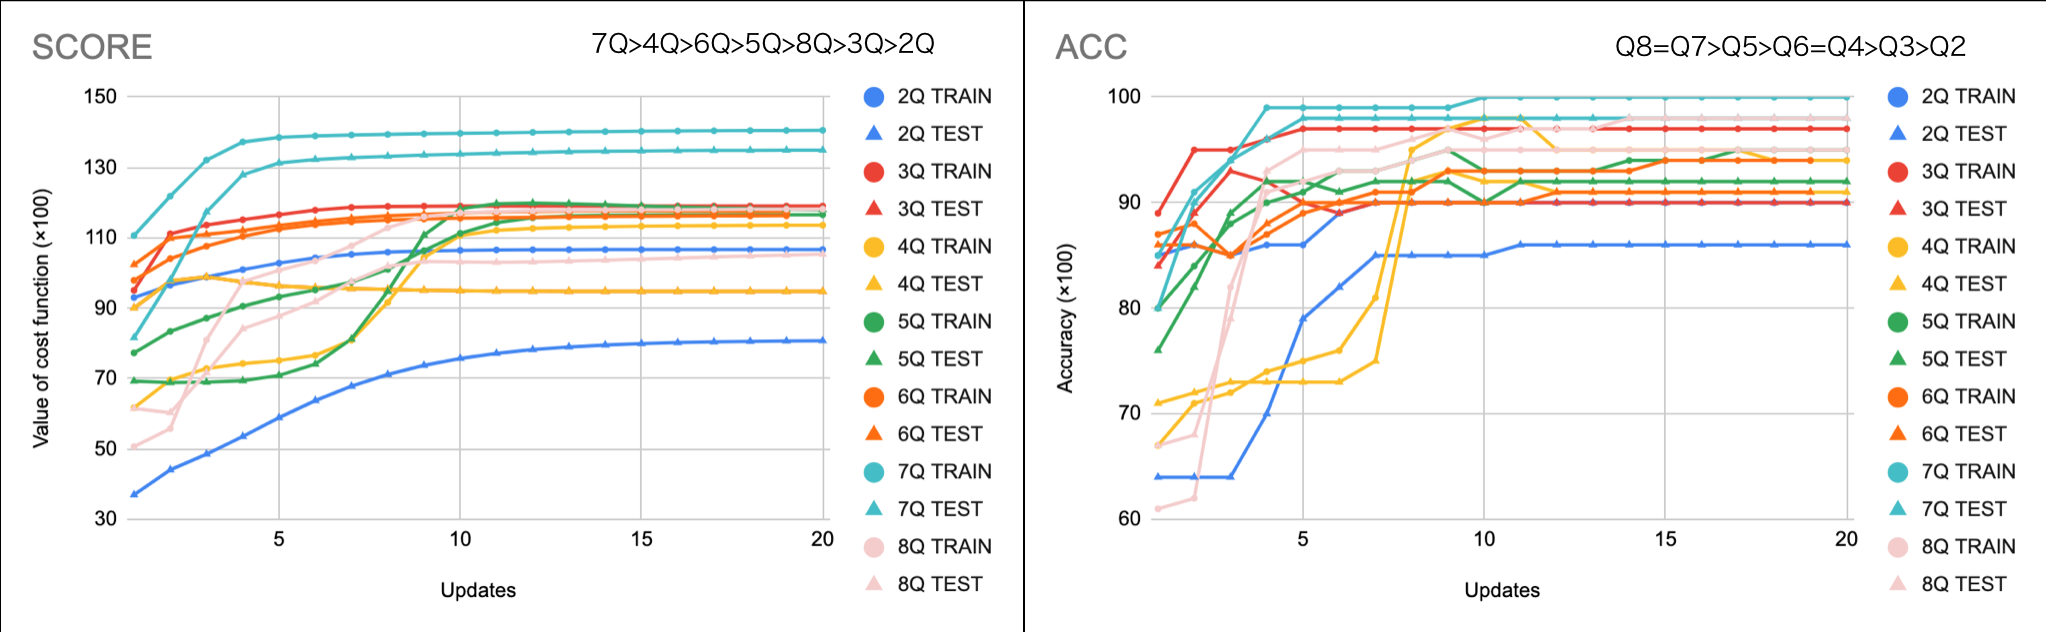
\includegraphics[keepaspectratio, scale=0.43]{experiment/figure/MNIST_qubit_change.png}
    \caption{MNIST classification with changed number of qubits. Fixed at 3 fraxis layers, 100 training and evaluation data.}
    \label{fig:MNIST_qubit_change}
\end{figure}
\begin{figure}[H]
    \centering
    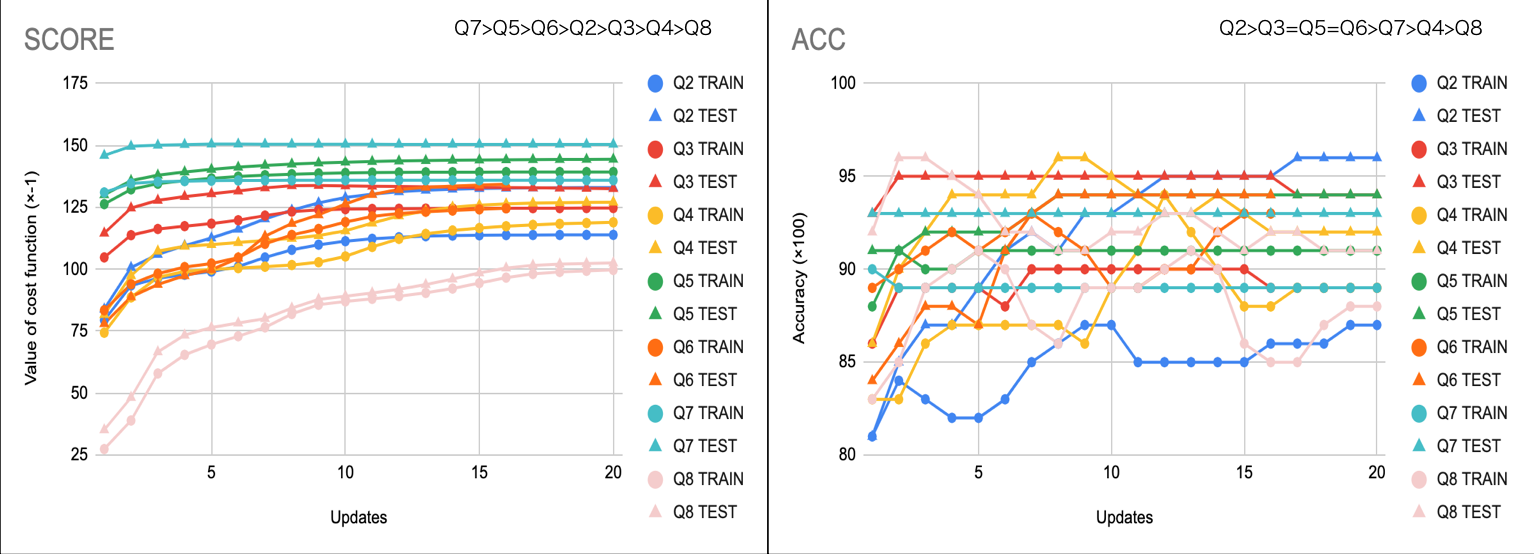
\includegraphics[keepaspectratio, scale=0.57]{experiment/figure/FMNIST_qubit_change.png}
    \caption{Fashioon-MNIST classification with changed number of qubits. Fixed at 3 fraxis layers, 100 training and evaluation data.}
    \label{fig:FMNIST_qubit_change}
\end{figure}

\par Figure \ref{fig:MNIST_qubit_change} indicates that more qubits result better, on the other hand, Figure \ref{fig:FMNIST_qubit_change} indicates the contrary. Generally speaking, more qubits result in more expressibility of the quantum circuit, so the quantum circuit with the more number of qubits should perform better than the circuit with less qubits. The results of \ref{fig:FMNIST_qubit_change} contradict this. It is thought that the increase in qubits (that is, the increase in fraxis gates, or the parameters to be optimized) made optimization difficult. In addition, even though training progresses, a temporary decrease in accuracy is observed.\\

\subsection{Change the number of fraxis layer}
Here, we show how the quantum circuit converges when the number of qubits is fixed at 2 and the number of fraxis layer is changed from 1 to 3. The number of the training data and the evaluation data are both fixed at 100. 

\begin{figure}[H]
    \centering
    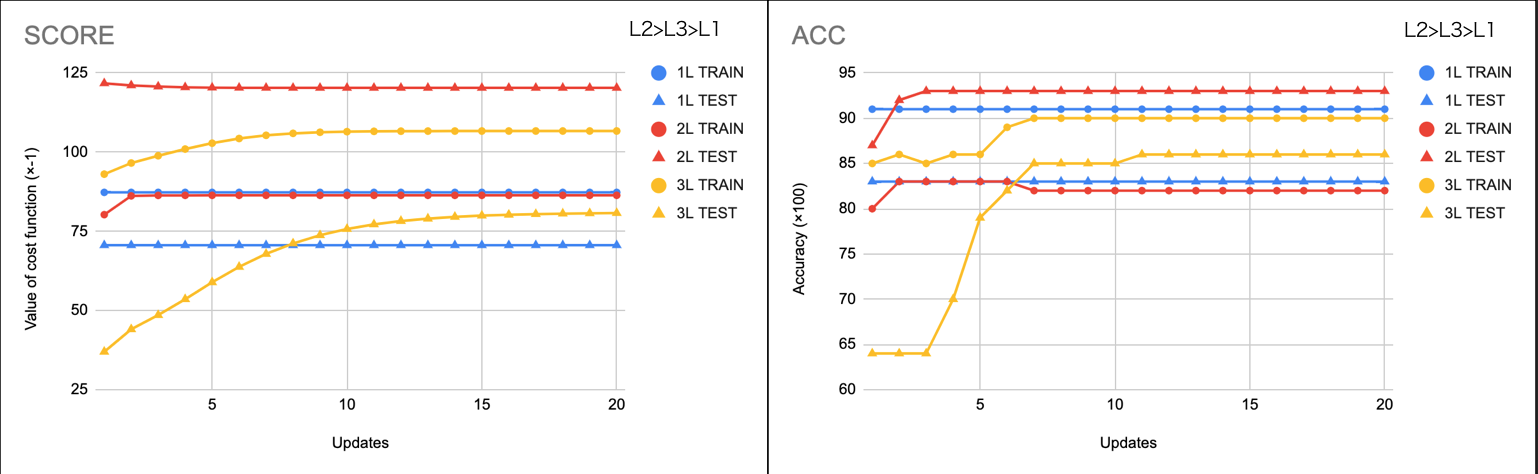
\includegraphics[keepaspectratio, scale=0.54]{experiment/figure/MNIST_layer_change.png}
    \caption{MNIST classification with changed number of fraxis layer. Fixed at 2 qubits, 100 training and evaluation data.}
    \label{fig:MNIST_layer_change}
\end{figure}
\begin{figure}[H]
    \centering
    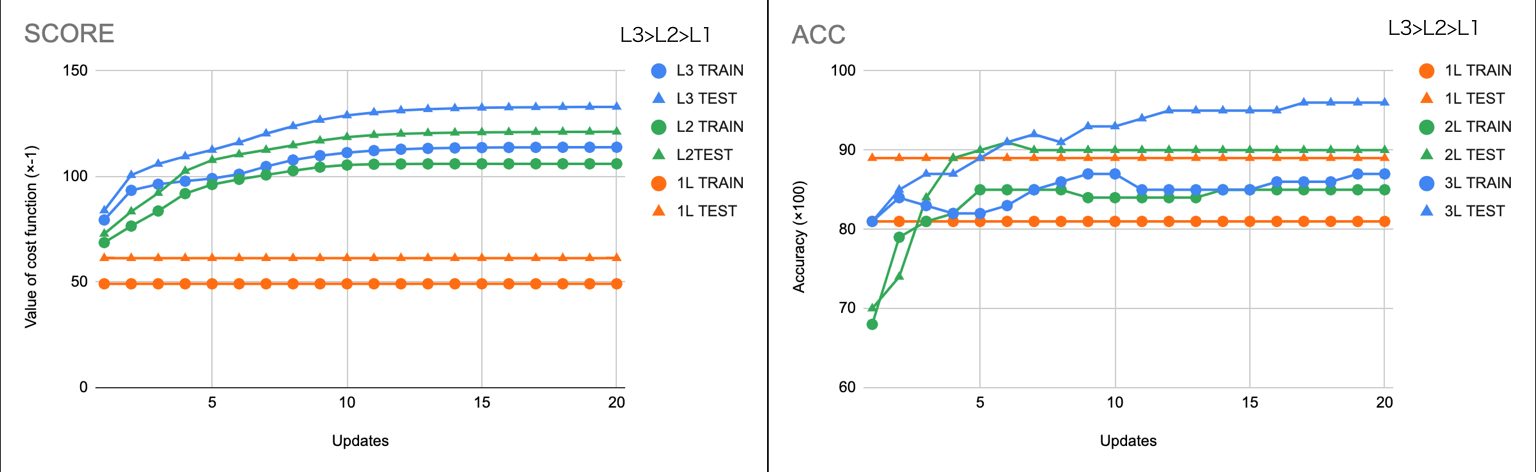
\includegraphics[keepaspectratio, scale=0.54]{experiment/figure/FMNIST_layer_change.png}
    \caption{Fashioon-MNIST classification with changed number of fraxis layer. Fixed at 2 qubits, 100 training and evaluation data.}
    \label{fig:FMNIST_layer_change}
\end{figure}

\par Figure \ref{fig:FMNIST_layer_change} indicates that more fraxis layers result better, on the other hand, Figure \ref{fig:MNIST_layer_change} indicates that more fraxis layer does not necessarily mean the better result. More layers mean the more parameters to be optimized, therefore, in general, result in better performance. The results of \ref{fig:MNIST_layer_change} do not follow this. It is thought that the increase in fraxis layers (that is, the increase in fraxis gates, or the parameters to be optimized) made optimization difficult. In addition, even though training progresses, a temporary decrease in accuracy is observed.\\

\subsection{Change the degree of parallelization}
Here we show how our algorithm can achieve the parallelization. We change the number of quantum nodes ny simulation from 1 to 3. The number of the training data and the evaluation data are both fixed at 100, the number of qubit is 6, and the number of fraxis layer is 3. The MNIST dataset is used.
\begin{figure}[H]
    \centering
    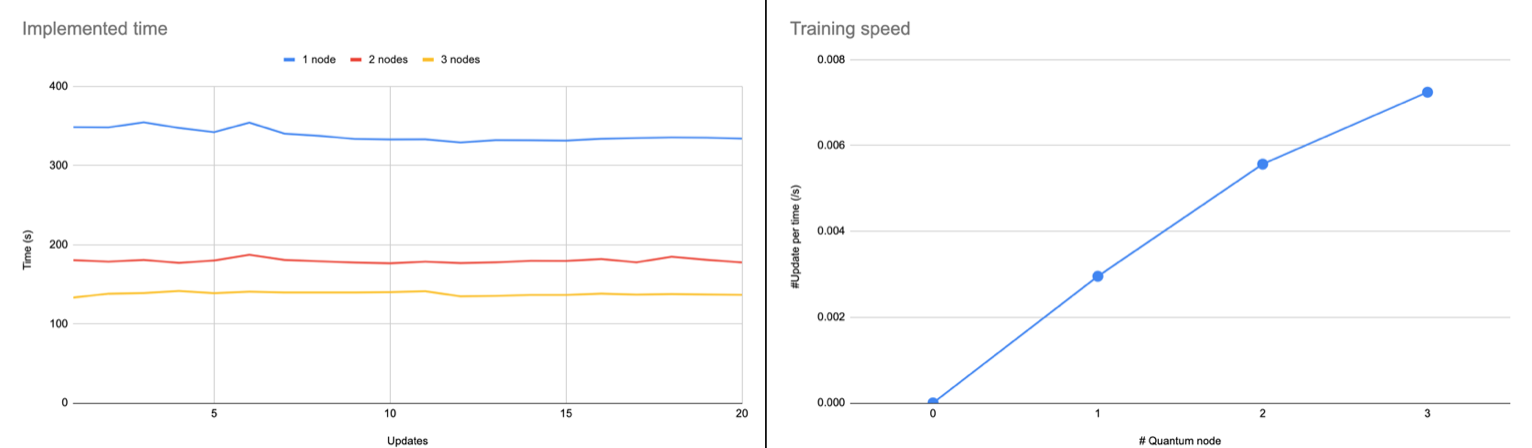
\includegraphics[keepaspectratio, scale=0.54]{experiment/figure/MNIST_node_change_time.png}
    \caption{MNIST classification with changed number of the quantum node. Fixed at 6 qubits, 3 fraxis layers, 100 training and evaluation data.}
    \label{fig:MNIST_node_change_time}
\end{figure}
\begin{figure}[H]
    \centering
    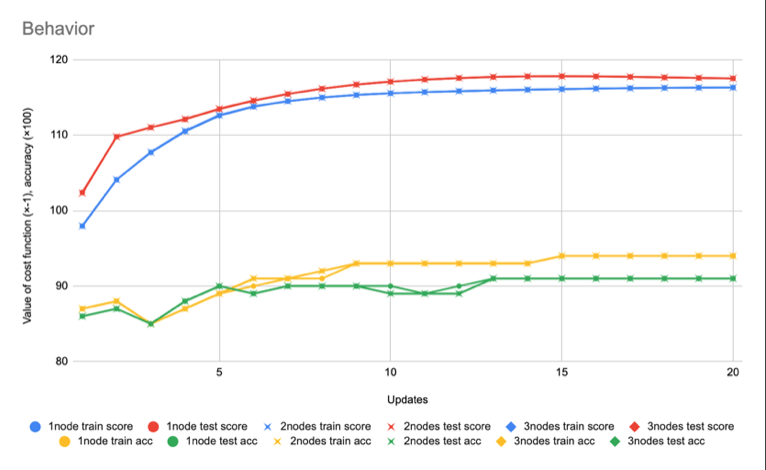
\includegraphics[keepaspectratio, scale=0.54]{experiment/figure/MNIST_node_change_behavior.png}
    \caption{MNIST classification with changed number of the quantum node. Fixed at 6 qubits, 3 fraxis layers, 100 training and evaluation data.}
    \label{fig:MNIST_layer_change_behavior}
\end{figure}

\par Figure \ref{fig:MNIST_node_change_time} indicates the parallelization achieves the speed up the training in almost linear-scale as shown theoretically above. Figure \ref{fig:MNIST_layer_change_behavior} indicates that the parallelization makes little change in behavior, but theoretically behavior of distributed algorithms (in which the number of quantum nodes is two or three) must completely match behavior of non-distributed one (in which the number of quantum nodes is one). These differences in behavior of algorithms is caused by precision loss. Our proposed parallelization scheme changes the order of addition (subtraction) calculations when aggregating and summing up the matrix $G^{(i)}$ to construct the matrix $G$. This change of the calculation order produces precision loss and minor differences between distributed algorithm and non-distributed one, which causes big differences in solving the eigenvector of the matrix $G$. 

\par In order to decrease the differences in behavior of the distributed algorithm from the non-distributed one, we tried ignoring 5 decimal places of the matrix $G$, from which the eigenvector is calculated. The minor differences of this matrix $G$ is the cause of the difference in behavior, and we thought of an operation to eliminate small differences in the matrix. The results of experiments are as follows.

\begin{figure}[H]
    \centering
    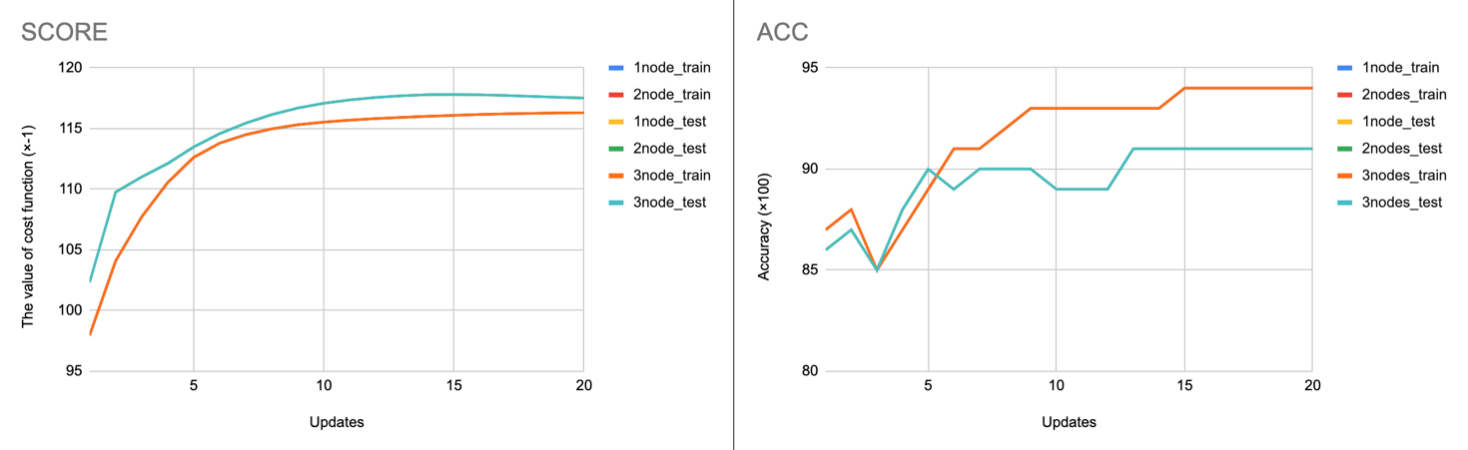
\includegraphics[keepaspectratio, scale=0.54]{experiment/figure/ignore_MNIST_node_change.png}
    \caption{MNIST classification with changed number of quantum node. Fixed at 6 qubits, 3 fraxis layers, 100 training and evaluation data. We ignored 5 decimal places of the matrix $G$.}
    \label{fig:ignore_MNIST_node_change}
\end{figure}

\par Figure \ref{fig:ignore_MNIST_node_change} shows exactly the same behavior of distributed algorithm from the non-distributed one.